\chapter{Quantum machine learning}

\section{Data encoding}

\section{Quantum neural networks}

\subsection{QNN versus NN}
Using the same data, model structure and optimiser as in \cite{abbas2021}, measuring instead performance using 10-fold cross validation, the quantum neural networks clearly outperform the classical. The mean accuracy during training is shown in \cref{fig:iris_training}. For simulation of noise, the 27-qubit IBM Montreal architecture was chosen, as it was the actual hardware used in \cite{abbas2021} The model with noise was only trained for ten epochs, due to the significant time required for the noisy simulation, but the results show that noise did not have a significant impact on the performance.

\begin{figure}
    \centering
    \begin{tikzpicture}
        \begin{axis}[
                width=0.8\textwidth,
                xlabel={Iteration},
                ylabel={Out of fold accuracy},
                grid = major,
                legend pos=south east,
                legend cell align={left},
            ]
            \addplot[mark=none, color=blue] table[x index=0, y index=3, col sep=comma] {../code/iris/results/mean.csv};
            \addplot[mark=none, color=red] table[x index=0, y index=2, col sep=comma] {../code/iris/results/mean.csv};
            \addplot[mark=none, color=green] table[x index=0, y index=1, col sep=comma] {../code/iris/results/mean.csv};
            \legend{
                Noisy QNN,
                Exact QNN,
                Classical NN
            }
        \end{axis}
    \end{tikzpicture}
    \caption{Mean accuracy during training for the Iris dataset using 10-fold cross validation.}
    \label{fig:iris_training}
\end{figure}

\subsection{Quantum convolutional neural networks}
Testing a QCNN on synthetic data shown in \cref{fig:qcnn_data}; classify pictures as either horizontal or vertical lines. The model without errors achieve 100\% accuracy on both training and test data, while the noisy model only managed around 90\% accuracy on the training data and 80\% on test data. The loss function of the noisy and exact model during training is shown in \cref{fig:qcnn_loss}.


\begin{figure}
    \centering
    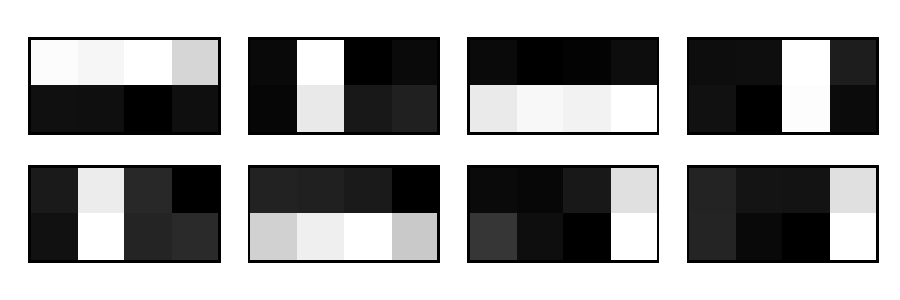
\includegraphics[width=0.8\textwidth]{../code/qcnn/data.pdf}
    \caption{Synthetic data for the QCNN.}
    \label{fig:qcnn_data}
\end{figure}


\begin{figure}
    \centering
    \begin{tikzpicture}
        \begin{axis}[
                width=0.8\textwidth,
                xlabel={Iteration},
                ylabel={Loss},
                % legend pos=north west,
                % legend style={at={(0.5,1.03)},anchor=north},
                grid=major,
            ]
            \addplot[mark=none, color=blue, width=] table[x index=0, y index=1, col sep=comma] {../code/qcnn/optim.csv};
            \addplot[mark=none, color=red] table[x index=0, y index=2, col sep=comma] {../code/qcnn/optim.csv};
            \legend{Noisy QCNN, Exact QCNN}
        \end{axis}
    \end{tikzpicture}
    \caption{Loss function of QCNN model during training with both exact simulations and noisy.}
    \label{fig:qcnn_loss}
\end{figure}


